\documentclass[11pt]{article}

\author{Math 123}
\date{Due March 3, 2023 by \emph{midnight} } 
\title{Homework 5}

\usepackage{graphicx,xypic}
\usepackage{amsthm}
\usepackage{amsmath,amssymb}
\usepackage{amsfonts}
\usepackage{xcolor}
\usepackage[margin=1in]{geometry}
\usepackage[shortlabels]{enumitem}
\newtheorem{problem}{Problem}
\renewcommand*{\proofname}{{\color{blue}Solution}}


\usepackage{fancyhdr}
\pagestyle{fancy}
\rhead{Math 123, Homework 5}

\setlength{\parindent}{0pt}
\setlength{\parskip}{1.25ex}

% tikz
\usepackage{tikz}
\usetikzlibrary{intersections, angles, quotes, positioning}
\usetikzlibrary{arrows.meta}
\usepackage{pgfplots}
\pgfplotsset{compat=1.13}


\tikzset{
	force/.style={thick, {Circle[length=2pt]}-stealth, shorten <=-1pt}
}

% quiver style
\usepackage{tikz-cd}
% `calc` is necessary to draw curved arrows.
\usetikzlibrary{calc}
% `pathmorphing` is necessary to draw squiggly arrows.
\usetikzlibrary{decorations.pathmorphing}

% A TikZ style for curved arrows of a fixed height, due to AndréC.
\tikzset{curve/.style={settings={#1},to path={(\tikztostart)
					.. controls ($(\tikztostart)!\pv{pos}!(\tikztotarget)!\pv{height}!270:(\tikztotarget)$)
					and ($(\tikztostart)!1-\pv{pos}!(\tikztotarget)!\pv{height}!270:(\tikztotarget)$)
					.. (\tikztotarget)\tikztonodes}},
	settings/.code={\tikzset{quiver/.cd,#1}
			\def\pv##1{\pgfkeysvalueof{/tikz/quiver/##1}}},
	quiver/.cd,pos/.initial=0.35,height/.initial=0}

% TikZ arrowhead/tail styles.
\tikzset{tail reversed/.code={\pgfsetarrowsstart{tikzcd to}}}
\tikzset{2tail/.code={\pgfsetarrowsstart{Implies[reversed]}}}
\tikzset{2tail reversed/.code={\pgfsetarrowsstart{Implies}}}
% TikZ arrow styles.
\tikzset{no body/.style={/tikz/dash pattern=on 0 off 1mm}}

\begin{document}

\maketitle

% You are required to put your name here:
{\bf\Large Name: George Chemmala} 


\vspace{.3in}
Topics covered: matchings, K\"onig's theorem, vertex covers, Gale--Shapely algorithm 

Instructions: 
\begin{itemize}
\item This assignment must be submitted on Gradescope by the due date. 
\item If you collaborate with other students (which is encouraged!), please mention this somewhere on the assignment. 
\item If you are stuck, please ask for help (from me, a TA, a classmate). Use Campuswire!  
\item You may freely use any fact proved in class. In general, you should provide proof for facts used that were not proved in class. 
\item {\bf Please restrict your solution to each problem to a single page.} Usually solutions can be even shorter than that. If your solution is very long, you should think more about how to express it concisely.
\end{itemize}

\pagebreak 



\begin{problem}
Let $G=(V,E)$ be a bipartite graph with maximum vertex degree $\Delta$. \begin{enumerate}[(a)]
\item Use K\"onig's theorem to prove that $G$ has a matching of size at least $|E|/\Delta$. 
\item Use (a) to conclude that every subgraph of $K_{n,n}$ with more than $(k-1)n$ edges has a matching of size at least $k$. 
\end{enumerate} 
\end{problem}

\begin{proof}
\begin{enumerate}
    \item[]
    \item[(a)] If the maximum vertex degree is \(\Delta\) then each vertex covers at most \(\Delta\) edges. Therefore, vertex cover must be at least of size \(|E| / \Delta\), so by König's Theorem the matching of the bipartite graph \(G\) must be at least size \(|E| / \Delta\)

    \item[(b)] The \(K_{n,n}\) graph has \(\Delta \leq n\) so \(|E|/\Delta > (k-1)n / n = k - 1\). Therefore, \(|E|/\Delta \geq k\) and by König's Theorem the matching must be at least size \(k\)  
\end{enumerate}
\end{proof}

\pagebreak



\begin{problem}
Fix $k\ge2$, and let $Q_k$ denote hypercube graph (from HW1). Prove that $Q_k$ has at least $2^{2^{k-2}}$ perfect matchings.
\end{problem}

\begin{proof}
By induction:

\emph{Base Case:} When \(k = 2\) we see that \(2^{2^{k-2}} = 2^{2^{0}} = 2^1 = 2\), and we know that there are \(2\) perfect matchings:

% https://q.uiver.app/?q=WzAsMTUsWzAsMSwiXFxidWxsZXQiXSxbMSwxLCJcXGJ1bGxldCJdLFswLDIsIlxcYnVsbGV0Il0sWzEsMiwiXFxidWxsZXQiXSxbMiwxLCJcXGJ1bGxldCJdLFsyLDIsIlxcYnVsbGV0Il0sWzMsMSwiXFxidWxsZXQiXSxbMywyLCJcXGJ1bGxldCJdLFs0LDEsImMiXSxbNSwxLCJcXGJ1bGxldCJdLFs0LDIsIlxcYnVsbGV0Il0sWzUsMiwiYyJdLFswLDAsIk1fMSJdLFsyLDAsIk1fMiJdLFs0LDAsIlZfYyJdLFswLDEsIiIsMCx7InN0eWxlIjp7ImJvZHkiOnsibmFtZSI6Im5vbmUifSwiaGVhZCI6eyJuYW1lIjoibm9uZSJ9fX1dLFsyLDMsIiIsMCx7InN0eWxlIjp7ImJvZHkiOnsibmFtZSI6Im5vbmUifSwiaGVhZCI6eyJuYW1lIjoibm9uZSJ9fX1dLFswLDIsIiIsMSx7InN0eWxlIjp7ImhlYWQiOnsibmFtZSI6Im5vbmUifX19XSxbMSwzLCIiLDEseyJzdHlsZSI6eyJoZWFkIjp7Im5hbWUiOiJub25lIn19fV0sWzQsNSwiIiwwLHsic3R5bGUiOnsiYm9keSI6eyJuYW1lIjoibm9uZSJ9LCJoZWFkIjp7Im5hbWUiOiJub25lIn19fV0sWzQsNiwiIiwyLHsic3R5bGUiOnsiaGVhZCI6eyJuYW1lIjoibm9uZSJ9fX1dLFs1LDcsIiIsMCx7InN0eWxlIjp7ImhlYWQiOnsibmFtZSI6Im5vbmUifX19XSxbNiw3LCIiLDIseyJzdHlsZSI6eyJib2R5Ijp7Im5hbWUiOiJub25lIn0sImhlYWQiOnsibmFtZSI6Im5vbmUifX19XSxbOCw5LCIiLDIseyJzdHlsZSI6eyJoZWFkIjp7Im5hbWUiOiJub25lIn19fV0sWzgsMTAsIiIsMCx7InN0eWxlIjp7ImhlYWQiOnsibmFtZSI6Im5vbmUifX19XSxbMTAsMTEsIiIsMCx7InN0eWxlIjp7ImhlYWQiOnsibmFtZSI6Im5vbmUifX19XSxbOSwxMSwiIiwyLHsic3R5bGUiOnsiaGVhZCI6eyJuYW1lIjoibm9uZSJ9fX1dXQ==
\[\begin{tikzcd}
	{M_1} && {M_2} && {V_c} \\
	\bullet & \bullet & \bullet & \bullet & c & \bullet \\
	\bullet & \bullet & \bullet & \bullet & \bullet & c
	\arrow[draw=none, from=2-1, to=2-2]
	\arrow[draw=none, from=3-1, to=3-2]
	\arrow[no head, from=2-1, to=3-1]
	\arrow[no head, from=2-2, to=3-2]
	\arrow[draw=none, from=2-3, to=3-3]
	\arrow[no head, from=2-3, to=2-4]
	\arrow[no head, from=3-3, to=3-4]
	\arrow[draw=none, from=2-4, to=3-4]
	\arrow[no head, from=2-5, to=2-6]
	\arrow[no head, from=2-5, to=3-5]
	\arrow[no head, from=3-5, to=3-6]
	\arrow[no head, from=2-6, to=3-6]
\end{tikzcd}\]

The fact the vertex cover \(V_c\) has only two vertices proves that these matchings (\(M_1\) and \(M_2\)) are perfect.

\emph{Inductive Step:}  When we have graph of size \(k\) we can recognize that there exist matchings of each \(k-1\) subgraph where they are independent of the other ones, and there are \(2^{2^{k-3}} \cdot 2^{2^{k-3}} = 2^{2^{k-3} + 2^{k-3}} = 2^{2 \cdot 2^{k-3}} = 2^{2^{k-2}}\). Therefore, with only counting the matchings arising from taking the subgraphs independent of each other we find that there must be at least \(2^{2^{k-2}}\) perfect matchings.
\end{proof}

\pagebreak



\begin{problem}
Determine the stable matchings resulting from the proposal algorithm run with cats proposing and with giraffes proposing, given the preference lists below.
\begin{center}
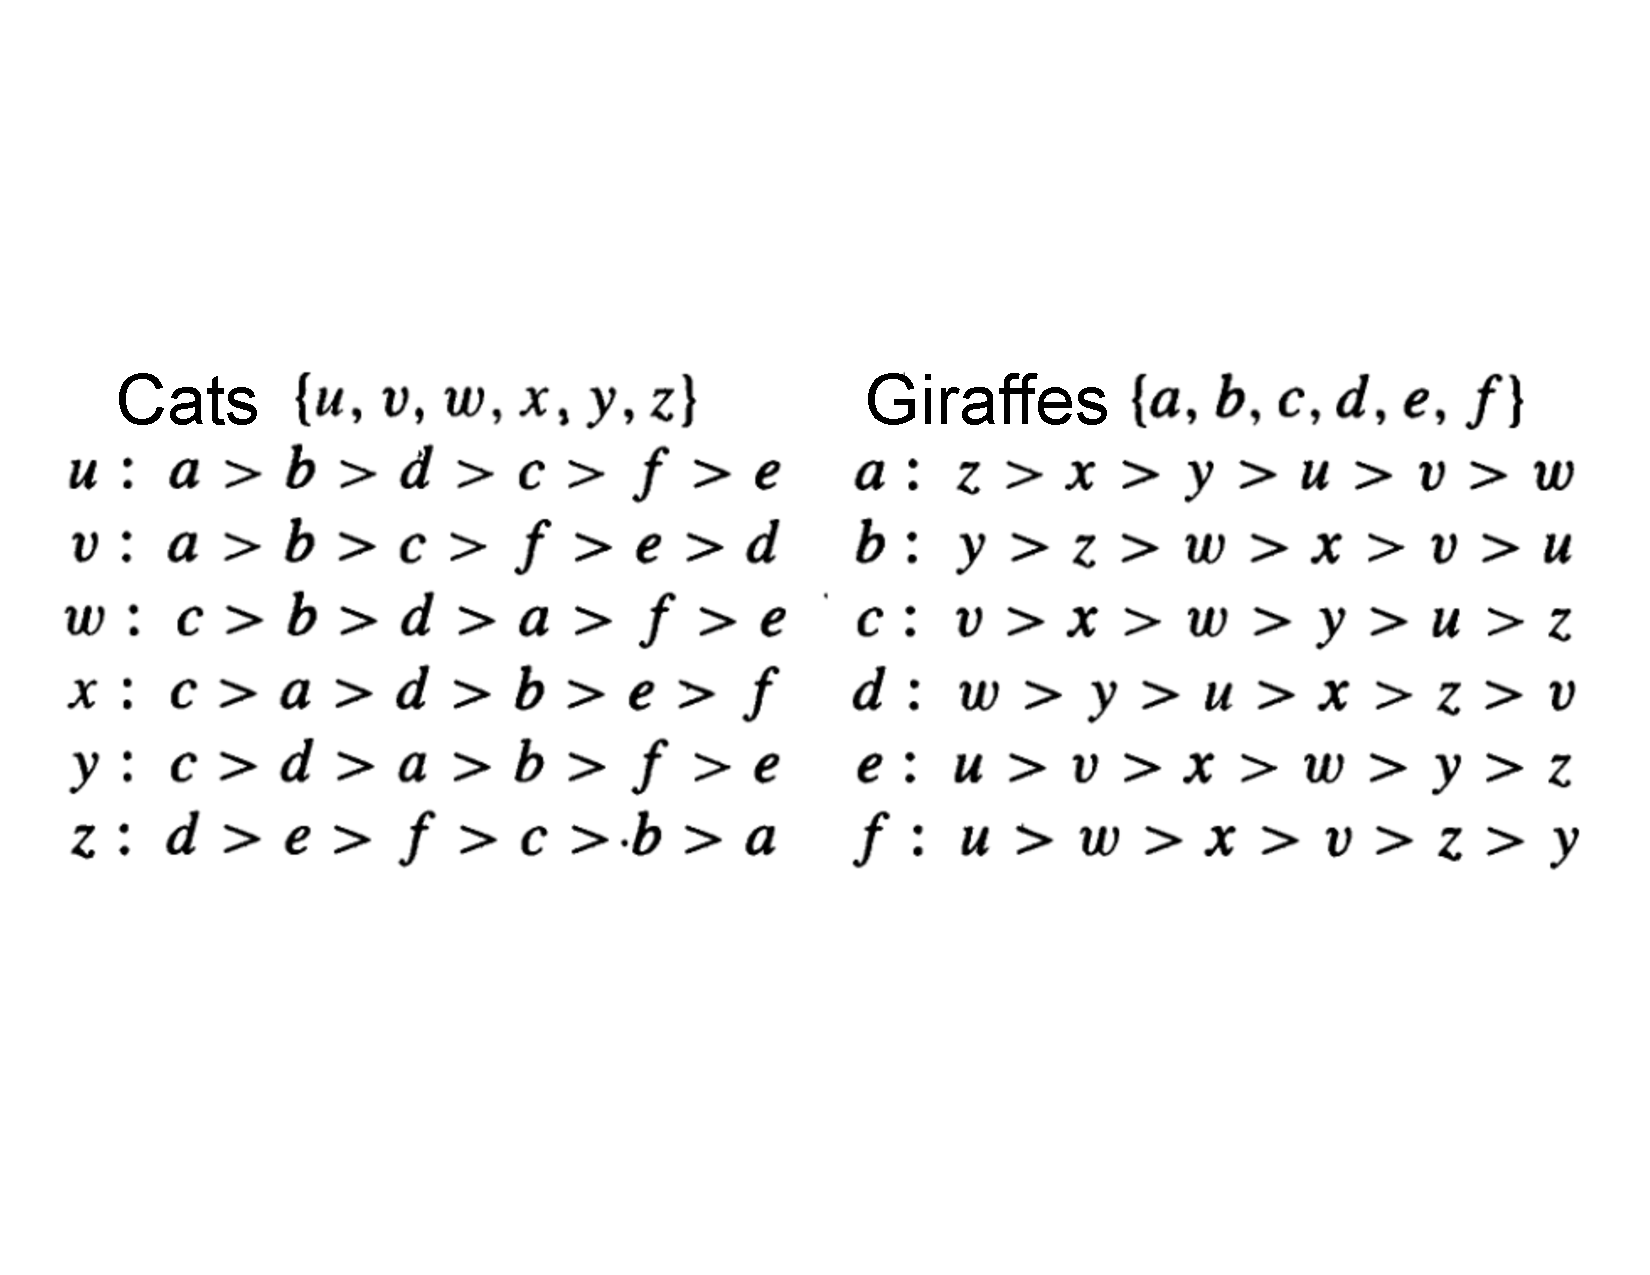
\includegraphics[scale=.5]{stable-match.pdf}
\end{center}
To receive full credit, you should show your work.
\end{problem}

\begin{proof}
    Let \(q \to r\) represent a proposal and \(q \not\to r\) represent a rejection.

    Cats \(\to\) Giraffes
    \begin{enumerate}
        \item \begin{enumerate}
            \item[P] \(u \to a, v \to a, w \to c, x \to c, y \to c, z \to d\) 
            \item[R] \(v \not\to a, w \not\to c, y \not\to c\) 
        \end{enumerate}
        \item \begin{enumerate}
            \item[P] \(u \to a, v \to b, w \to b, x \to c, y \to d, z \to d\) 
            \item[R] \(v \not\to b, z \not\to d\) 
        \end{enumerate}
        \item \begin{enumerate}
            \item[P] \(u \to a, v \to c, w \to b, x \to c, y \to d, z \to e\) 
            \item[R] \(x \not\to c\) 
        \end{enumerate}
        \item \begin{enumerate}
            \item[P] \(u \to a, v \to c, w \to b, x \to a, y \to d, z \to e\) 
            \item[R] \(u \not\to a\) 
        \end{enumerate}
        \item \begin{enumerate}
            \item[P] \(u \to b, v \to c, w \to b, x \to a, y \to d, z \to e\) 
            \item[R] \(u \not\to b\) 
        \end{enumerate}  
        \item \begin{enumerate}
            \item[P] \(u \to d, v \to c, w \to b, x \to a, y \to d, z \to e\) 
            \item[R] \(u \not\to d\) 
        \end{enumerate}
        \item \begin{enumerate}
            \item[P] \(u \to c, v \to c, w \to b, x \to a, y \to d, z \to e\) 
            \item[R] \(u \not\to c\) 
        \end{enumerate} 
        \item \begin{enumerate}
            \item[P] \(u \to f, v \to c, w \to b, x \to a, y \to d, z \to e\) 
            \item[R] None, therefore the computation is complete 
        \end{enumerate}  
    \end{enumerate}
    
    Giraffes \(\to\) Cats
    \begin{enumerate}
        \item \begin{enumerate}
            \item[P] \(a \to z, b \to y, c \to v, d \to w, e \to u, f \to u\) 
            \item[R] \(e \not\to u\) 
        \end{enumerate}
        \item \begin{enumerate}
            \item[P] \(a \to z, b \to y, c \to v, d \to w, e \to v, f \to u\) 
            \item[R] \(e \not\to v\) 
        \end{enumerate}
        \item \begin{enumerate}
            \item[P] \(a \to z, b \to y, c \to v, d \to w, e \to x, f \to u\) 
            \item[R] None, therefore the computation is complete 
        \end{enumerate}  
    \end{enumerate}
\end{proof}

\pagebreak

\begin{problem}
Let $G=(X\sqcup Y,E)$ be a bipartite graph satisfying $|N(S)|>|S|$ for each nonempty $S\subset X$. Prove that every edge of $G$ belongs to some matching that saturates $X$. 
\end{problem}

\begin{proof}
By induction:

\emph{Base Case:} \(|E| = 1\)
Therefore, there is only one matching between \(\{x, y\}\) where \(x \in X\) and \(y \in Y\). This saturates \(x\)   

\emph{Inductive Step:} We know from Hall's Theorem that given $G=(X\sqcup Y,E)$, a bipartite graph satisfying $|N(S)| \geq |S|$ for each nonempty $S\subset X$ every edge of $G$ belongs to some matching that saturates $X$. Therefore, by removing an edge we now have a graph with \(n-1\), so by induction we can see that the remaining graph has some matching that saturates \(X\) 

\end{proof}

\pagebreak 

\begin{problem}
Complete the proof of K\"onig's theorem that we started in class. 
\end{problem}

\begin{proof}
    Let $G=(X\sqcup Y, E)$ be a bipartite graph, and let
    $M$ be a maximum matching. To prove the theorem, it suffices to find a vertex cover $Q$ with one vertex from each edge of $M$.
    
    Define $Q$ as follows. Given an edge $e=\{x,y\}$ of $M$ (here $x\in X$ and $y\in Y$), if there is an M-alternating path from an unsaturated vertex $u\in X$ that passes through $e$, then we put $y\in Q$. Otherwise we put $x\in Q$.
    
    We want to show that $Q$ is a vertex cover. Let $f=\{a,b\}$ be an edge of E, and assume $a\in X$ and $b\in Y$. If f is in M we are done, so assume not. Since M is maximum, at least one of a or b is saturated by some edge $e={x,y}$ in M. Now consider cases depending on whether $a=x$ or $b=y$ and whether or not there is an M-alternating path starting from an unsaturated vertex of $u\in X$ and passing through e.

    \begin{enumerate}
        \item\(a = x, b = y\) and there exists an M-alternating path - By definition \(y\) must be in \(Q\); therefore \(f\) is covered

        \item\(a = x, b = y\) and there doesn't exist an M-alternating path - By definition \(x\) must be in \(Q\); therefore \(f\) is covered 

        \item\(a = x\) and there exists an M-alternating path - Suppose \(b\) is not saturated then there would be an M-augmenting path connecting \(u\) and \(b\), a contradiction since \(M\) is maximal. Since \(b\) is in the matching then let \(e^\prime\) be the edge of \(M\) connected to \(b\) and \(c\). Therefore, \(c \in Q\) 

        \item\(a = x\) and there doesn't exist an M-alternating path - Let \(e^\prime  = \{b, c\} \in M\). Suppose there exists an M-alternating path s.t. it connected \(b\) to an unsaturated vertex, then the path could contain \(e\), a contradiction. Therefore, \(e^\prime\) cannot be in an  M-alternating path, so \(a = x \in Q\)

        \item\(b = y\) and there exists an M-alternating path - By definition \(y\) must be in \(Q\); therefore \(f\) is covered 

        \item\(b = y\) and there doesn't exist an M-alternating path - Let \(e^\prime\) be the edge of \(M\) connected to \(b\) and \(c\). Suppose, there exists an M-alternating path from \(u\) to \(e^\prime \) then there would be an M-alternating path from \(u\) to \(e\), a contradiction. Therefore, \(c \in Q\)  
    \end{enumerate}
\end{proof}

\pagebreak
\begin{problem}
A deck with $mn$ cards with $m$ values and $n$ suits consists of one card for each value in each suit. The cards are dealt into an $n\times m$ array. Prove that there is a set of $m$ cards, one in each column, having distinct values. 
\end{problem}

\begin{proof}
Let \(G\) be a bipartite graph with vertex set \(X \sqcup Y\) where \(x \in X\) are columns in the array and \(y \in Y\) are the distinct values and \(E\) is the edge set where \(e \in E\) correspond to value \(y\) appearing in a column \(x\). Each column consists of \(n\) cards and each value appears in \(n\) times in total, so the graph is \(n\)-regular, meaning we can apply the Marriage Theorem (a corollary of Hall's Theorem), so see that there is a perfect matching which shows that there is a set of $m$ cards, one in each column, having distinct values.
\end{proof}

\pagebreak


\pagebreak

\begin{problem}[Bonus]
Let $T_1$ be the tiling of the plane by unit squares whose vertices have integer coordinates. Let $T_2$ be the result of rotating $T_1$ about the origin by some angle $\theta$. Prove that it is possible to find a bijection between squares of $T_1$ and squares of $T_2$ in such a way that the matched squares are within 10 units of each other. The matching will depend on $\theta$. 
\end{problem}


\begin{proof}

\end{proof}


\end{document}